% SVN info for this file
\svnidlong
{$HeadURL$}
{$LastChangedDate$}
{$LastChangedRevision$}
{$LastChangedBy$}

\chapter{Dalla legge di Coulomb al formalismo dei campi vettoriali}
\labelChapter{ellipseintroduction}

\begin{introduction}
‘‘Per ogni problema c'è una soluzione che è semplice, chiara... e sbagliata.''
\begin{flushright}
	\textsc{Henry Louis Mencken} ad un suo studente che trovò come perimetro dell'ellisse $\pi ab$. % TO DO: quote 
\end{flushright}
\end{introduction}
\lettrine[findent=1pt, nindent=0pt]{L}{a meccanica} ci descrive come funziona un sistema soggetto ad una certa \textit{forza}. Ad oggi, siamo riusciti a ricondurre tutte le forze ad alcune \textbf{interazioni fondamentali}; in ordine di magnitudine decrescente:
 \begin{itemize}
 	\item (Nucleare) Forte.
 	\item Elettromagnetica.
 	\item (Nucleare) Debole
 	\item Gravitazionale
 \end{itemize}
\parshape=0 Wow, sono \textit{davvero} poche! Dov'è la frizione, la forza elastica, le reazioni vincolari, le forze chimiche che legano le particelle, gli urti tra palle del biliardo? Che ci crediate o no, \textit{tutte} queste forze sono elettromagnetiche. E le altre interazioni fondamentali che fine fanno?

Le \textbf{interazioni (nucleari) forti} tengono uniti i \textit{quark} che costituiscono neutroni e protoni, nonché legano assieme protoni e neutroni nel \textit{nucleo atomico}, ma agiscono su una scala così piccola che risultano essere completamente impercettibili - pur essendo centinaia di volte più forti delle forze elettromagnetiche!\\
Le \textbf{interazioni (nucleari) deboli}, che riguardano certi procedimenti di decadimenti nucleari, hanno un nome autoesplicativo: sono forze a microscopico raggio d'azione \textit{e} sono più deboli delle forze elettromagnetiche.\\
Non parliamo poi della \textbf{interazione gravitazionale}: essa è terribilmente debole nonostante abbia un \textit{range} d'azione infinito, e la notiamo solamente in presenza di grandi, \textit{enormi} concentrazioni di massa - i pianeti e le stelle. Se al posto delle forze elettriche l'atomo fosse tenuto assieme da forze gravitazionali, un singolo atomo di idrogeno sarebbe più grande dell'intero universo osservabile.

Quindi, non solo le \textbf{forze elettromagnetiche} sono quelle dominanti nella vita di tutti i giorni (sono potenti \textit{e} hanno un \textit{range} d'azione infinito), ma sono anche le sole che \textit{al momento} sono completamente spiegate da una teoria. Certo, c'è una teoria gravitazionale classica e relativistica, ma non ne esiste una soddisfacente in campo quantistico; per le forze deboli c'è una teoria popolare, ma ostica, e per le forti si sta facendo strada la \textit{cromodinamica}... eppure, nessuna di queste teorie può vantare una verifica sperimentale definitiva. La cosa curiosa è che tutte queste teorie sperimentali si rifanno al modello perfetto, da emulare, delle \textit{leggi (classiche) dell'elettromagnetismo}.

Anche se le prime osservazioni sui fenomeni elettromagnetici sono attribuite al filosofo greco Talete nel VI secolo a.C., fu grazie alle innumerevoli scoperte di Franklin, Coulomb, Ampère, Faraday, Volta e tanti altri che \textbf{James Clerk Maxwell} impacchettò tutto questo bagaglio scientifico in quattro, stupende formule matematiche - che probabilmente avrete visto per la prima volta su una discutibile maglietta di un fan sfegatato della Fisica.

Prima di arrivare a formulare tutte le equazioni di Maxwell, tuttavia, ci conviene fare un tour guidato attraverso la storia di questa disciplina, costruendo passo per passo queste leggi facendo le stesse osservazioni dei più famosi scienziati che lavorarono sull'elettromagnetismo - chiaramente, viste con degli strumenti matematici moderni. In questo capitolo, dopo un'excursus storico dello studio dei fenomeni elettrostatici introdurremo la \textbf{legge di Coulomb}; la seconda parte sarà più prettamente matematica e tratterà del \textbf{formalismo dei campi vettoriali} - introducendo diversi strumenti particolarmente utili ai nostri scopi.
\section{I primi studi dell'elettricità}
Già, ma... che significa il termine \textbf{‘‘elettromagnetismo''}? La sua etimologia permette di svelare molte informazioni su come stati osservati in natura questi fenomeni:
\begin{itemize}
	\item ‘‘Elettro'' e ‘‘elettricità'' derivano da \textit{elettricus}, parola latina coniata nel 1600 da \textbf{William Gilbert} nel suo trattato \textit{De Magnete}, derivata a sua volta dal termine \textit{elektron}, ‘‘ambra'' in greco: infatti, le popolazioni attorno al Mediterraneo sapevano che oggetti in ambra, se strofinati con il pelo di gatto o col vello di lana, erano in grado di attrarre oggetti leggeri come piume e pagliuzze.
	\item ‘‘Magnetismo'' deriva da \textit{magnētis lithos}, ‘‘pietra di Magnesia'' in greco: sull'isola egea di Magnesia erano diffuse rocce di \textit{magnetite}, un minerale ferroso che in certi casi è capace di attrarre piccoli pezzetti di ferro.
\end{itemize}
\paragraph{Elettrizzazione per strofinio}
Il già citato Gilbert fu il primo a dare un certo rigore allo studio di questi fenomeni. Sperimentando sistematicamente con vari materiali, egli descrisse gli effetti delle \textbf{azioni elettriche per strofinio}\index{elettrizzazione per strofinio} - anche noto come \textbf{effetto triboelettrico}) - come segue:\\
\begin{minipage}{0.65\textwidth}
\begin{enumerate}[label=\alph*)]
	\item Due oggetti della \textit{stessa sostanza}, dopo essere stati strofinati da un panno, si \textit{respingono} se sono vicini l'un l'altro.
	\item Due oggetti di \textit{sostanze diverse} possono \textit{attrarsi} o \textit{respingersi}, a seconda dei materiali presi; ad esempio, vetro e ambra si attraggono.
	\item Due oggetti che sono attratti separatamente da un terzo oggetto si respingeranno a vicenda.
	\item Un oggetto è attratto da un materiale e un'altro oggetto è respinto da quel materiale, allora i due oggetti si attraggono tra di loro.
\end{enumerate}
\end{minipage}\hspace{10pt}
\begin{minipage}{0.34\textwidth}
		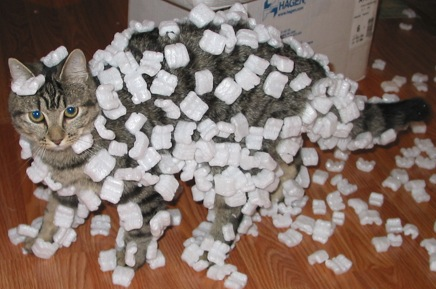
\includegraphics[width=1\textwidth]{images/foamcat.jpg}
	{\footnotesize Gilbert controllò tante combinazioni di materiali, ma non ‘‘pelo di gatto'' e ‘‘polistirolo da imballaggio''. Immagino non avesse un gatto per farlo.}
\end{minipage}\vspace{3pt}\\
Da queste osservazioni Gilbert concluse l'esistenza di due tipi diversi di elettrizzazione, attribuite a \textbf{cariche elettriche}\index{carica elettrica} differenti.
\begin{define}[Carica elettrica positiva e negativa]
	Convenzionalmente, si dice che:
	\begin{itemize}
		\item Corpi come il vetro acquisiscono carica elettrica \textbf{positiva}\index{carica elettrica!positiva}, indicata con il segno più ($+$).
		\item Corpi come l'ambra acquisiscono carica elettrica \textbf{negativa}\index{carica elettrica!negativa}, indicata con il segno meno ($-$).
	\end{itemize}
Sintetizzando quanto detto:
\begin{itemize}
	\item Cariche elettriche \textit{dello stesso segno} ($+/+,\ -/-$) si \textbf{respingono}.
	\item Cariche elettriche \textit{di segno opposto} ($+/-$) si \textbf{attraggono}.
\end{itemize}
\end{define}
Il buon vecchio Gilbert si accorse anche che, seppur esistevano materiali (ambra, vetro, ebanite, bachelite...) che venivano elettrizzati per strofinio, altri (metalli, il corpo umano...)\textit{non} venivano proprio elettrizzati. I primi li chiamò \textbf{isolanti}\index{isolante}, i secondi \textbf{conduttori}\index{conduttore}.
\paragraph{La struttura della materia e i fenomeni elettrostatici}
Gilbert scrisse per bene tutte queste osservazioni nel suo trattato \textit{De Magnete}, scritto nel 1600: all'epoca non poteva spiegare \textit{perché} succedeva ciò che aveva descritto, ma noi grazie alla conoscenza della \textit{struttura microscopica della materia} possiamo farlo. Senza perderci in tanti dettagli, la materia è fatta di \textbf{atomi}\index{atomo}, tutti costituiti da tre particelle: \textbf{protoni} $p$, \textbf{neutroni} $n$ ed \textbf{elettroni} $e$, rispettivamente di massa
\begin{itemize} % TO DO: simboli SI
	\item $m_p = 1,6725 \cdot 10^{-27}\ $ 
	\item $m_n = 1,6748\cdot 10^{-27}\ $
	\item $m_e = \frac{1}{1840}m_p=9,1091\cdot 10^{-31}\ $
\end{itemize}
Riprendendo la convenzione precedente, si vede che il protone ha carica \textit{positiva}, mentre l'elettrone ha carica \textit{negativa} e il neutrone non ha carica elettrica; ad oggi non è osservata alcuna carica elettrica più piccola di quella del protone o dell'elettrone - in altre parole, la carica elettrica è una grandezza \textbf{quantizzata}\footnote{La quantizzazione della carica è evidente a livello atomico e subatomico, ma diventa inapprezzabile se la non riescono a misurare variazioni dell'ordine della carica elementare - sperimentalmente si è visto intorno per carica sopra i $200 e$. Negli esperimenti normali di elettrostatica la carica è di fatto una quantità continua.}. Indicheremo con $-e$ la carica dell'elettrone e, in virtù della quantizzazione della carica elettrica, la chiameremo \textbf{carica elementare}\index{carica!elementare}, mentre con $+e$ indicheremo la carica del protone.

Il \textbf{nucleo}\index{nucleo}, costituito da protoni e neutroni, sta saldamente assieme grazie all'interazione nucleare forte che sovrasta le azioni repulsive delle cariche positive, che tra l'altro rendono il nucleo \textit{carico positivo}. Attorno al nucleo orbitano, attratte da forze elettriche, gli \textit{elettroni}: queste particelle sono in numero pari al numero di protoni nel nucleo e, a differenza di essi, sono molto più liberi di muoversi nello spazio circostante il nucleo. Si osserva che l'atomo è, nel suo complesso, \textit{elettricamente neutro}, dato che la carica del protone e dell'elettrone è uguale in modulo e la carica complessiva. Questo è estremamente importante per la struttura della materia; se non ci fosse questa \textit{cancellazione}\footnote{Per cancellazione non intendiamo che le carica si annichiliscono fisicamente, ma che i loro effetti si compensano, non producendo alcuna interazione ‘‘esterna''.} della carica, saremmo soggetti a forze estreme: una patata esploderebbe violentemente se ci fosse anche solo una cancellazione imperfetta dell'ordine di una parte su $10^10$.

Sostanze diverse hanno legami più o meno deboli tra il nucleo e gli elettroni, in particolari quelli periferici. Cosa succede, a livello microscopico, con l'elettrizzazione per strofinio? Il \textbf{contatto} tra i due corpi trasferisce \textit{per mezzo meccanico} elettroni dello strato superficiale da un corpo all'altro, dal corpo in cui sono meno fortemente legati verso quello in cui lo sono di più.
\begin{itemize}
	\item Negli \textbf{isolanti}, le cariche trasferite per strofinio rimangono \textit{localizzate}. Gli isolanti \textbf{non} trasportano facilmente la carica.
	\item Nei \textbf{conduttori}, le cariche elettriche negative sono \textit{libere di muoversi} e \textbf{non} rimangono localizzate. I conduttori trasportano facilmente la carica.
\end{itemize}
In altre parole, le forze elettriche sono una manifestazione fondamentale delle particelle atomiche (cariche) che costituiscono la materia, ma si manifestano a livello \textit{macroscopico} quando viene disturbata la simmetria naturale tra cariche positive e negative presenti negli atomi. Possiamo, in particolare, enunciare il seguente principio.
\begin{principle}[Principio della conservazione della carica]
	 Poiché la \textit{carica totale} di un corpo è data dalla \textit{somma algebrica} di tutte le cariche, in un sistema \textit{elettricamente isolato} la carica totale rimane costante nel tempo, ossia si \textit{conserva}.
\end{principle}
\paragraph{Induzione elettrostatica}
L'effetto triboelettrico che abbiamo visto è un caso particolare di \textbf{elettrizzazione per contatto}; tuttavia, si possono caricare corpi anche senza alcun contatto diretto, come accade con l'\textbf{induzione elettrostatica}\index{induzione elettrostatica}\\
Avviciniamo ad un \textit{conduttore} $C$, preso elettricamente scarico e sostenuto da un supporto isolante, un corpo carico $D$ - ad esempio, carico positivamente.
Il corpo carico esercita delle \textit{forze elettriche} sulle cariche microscopiche presenti sul conduttore; gli \textit{elettroni} nel conduttore sono liberi di muoversi sulla superficie e si dispongono nella zona di $C$ \textit{più vicina} al corpo carico, mentre la parte del conduttore più distante da $D$ risulterà carica positivamente\footnote{Chiaramente, se il corpo $D$ fosse carico negativamente accaderebbe l'opposto: gli elettroni in $C$ sarebbero respinti per l'interazione elettrica e si disporrebbero lontani dal corpo carico, rendendo positiva la zona vicina a $D$.}.
La carica complessiva del conduttore è, per conservazione della carica, sempre nulla, ma le cariche sono distribuite in modo non uniforme: convenzionalmente, pur essendo l'eccesso di cariche positive in una parte del conduttore dovuto al moto delle cariche negative, diremo che le cariche positive si sono spostate nella zona di $C$ a maggior distanza da $D$.

Se collegassimo il conduttore $C$ ad un conduttore $T$ molto più esteso di $C$, ad esempio la Terra, di fatto si creerebbe un unico conduttore $C+T$ praticamente infinito per i nostri scopi. In questo caso, le cariche positive si allontanerebbero molto da $D$; se interrompessimo il collegamento del conduttore a $T$ il conduttore $C$ resta carico negativamente - basta allontanare $D$ per ottenere $C$ negativo con distribuzione uniforme di carica.
\paragraph{Misura delle cariche elettriche: l'elettroscopio a foglie}
Abbiamo detto che la carica elettrica è una grandezza quantizzata... ma non abbiamo ancora parlato di come definirla esattamente, né di come \textit{misurarla}! Al momento, ne diamo una definizione operativa, tramite l'\textbf{elettroscopio a foglie}\index{elettroscopio a foglie}\\
Dato un contenitore isolante e trasparente si consideri un asta metallica che lo penetra in un foro in modo da rimanere bloccata. All'estremità inferiore, internamente al recipiente, sono appese due sottilissime foglioline metalliche - generalmente d'oro - liberi di ruotare attorno all'asse orizzontale dell'asta. Se l'asta metallica è scarica, le foglioline sono verticali per effetto della gravità.

Toccando l'asta con un corpo carico, essa si carica e parte della corrente posseduta dall'asta si dispone sulle foglioline. Poiché le foglioline sono cariche dello stesso segno, si respingono e divergono dalla verticale di un angolo $\alpha$ che può opportunamente misurato con una scala graduata: abbiamo creato uno strumento in grado di rilevare la presenza di cariche elettriche. Possiamo allora dare la seguente definizione \textit{operativa} di carica elettrica.
\begin{define}[Definizione operativa di carica elettrica]
Se due corpi uguali, toccando l'asta di un elettroscopio a foglie inizialmente scarico, fanno ruotare le foglioline di uno stesso angolo $\alpha$, allora hanno la stessa carica $q$.
\end{define}
Potremmo fornire già in questa maniera un'opportuna unità di misura, ma non è particolarmente utile e non è compatibile con la filosofia di molti sistemi di unità di misura. Tuttavia, per dare una possibile definizione \textit{non} operativa, dobbiamo quanto meno parlare dell'interazione elettrostatica.
\section{Legge di Coulomb}
Corpi carichi si attraggono o si respingono, a qualunque distanza, a seconda della loro carica: più sono vicini e più sono carichi, maggiore è questa attrazione/repulsione. Questa descrizione qualitativa delle forze di natura elettrostatica era già nota da Gilbert, ma per averne una \textit{quantitativa} dobbiamo aspettare quasi duecento anni.
Nel 1785, il fisico francese \textbf{Charles Augustin de Coulomb} pubblicò la sua memoria \textit{Recherches théoriques et expérimentales sur la force de torsion et sur l'élasticité des fils de metal}, in cui stabilì, mediante l'uso di una bilancia di torsione analoga a quella di \textit{Cavendish} per la misura delle forze gravitazionali, una legge matematica per la descrizione dell'interazione elettrostatica.
\begin{define}[Legge di Coulomb]\index{Legge!di Coulomb}
	Date due cariche puntiformi $q_1$ e $q_2$, poste a distanza $r$ \textit{nel vuoto}, interagiscono con una forza $F$ diretta secondo la loro congiungente data da
	\begin{equation}
		\vba{F}=k\frac{q_1q_2}{r^2}\vbh{u}_r\label{leggeCoulomb}
	\end{equation}
\end{define}
\begin{observes}~
	\begin{itemize}
		\item $\vba{F}$ è la forza che $q_1$ esercita su $q_2$; la forza che $q_2$ esercita su $q_1$ e $-\vba{F}$.
		\item $k$ è una costante di proporzionalità detta \textbf{costante di Coulomb}\index{costante!di Coulomb} che dipende dalle unità di misura.
		\item $\vbh{u}_r$ è il versore del vettore distanza $\vba{r}$ dalla carica $q_1$ alla carica $q_2$.
		\item $q_1q_2$ è il prodotto delle due cariche: se hanno lo stesso segno, la forza è repulsiva perché $\vba{F}$ ha lo stesso verso di $\vbh{u}_r$, altrimenti se hanno segno opposto è attrattiva perché hanno versi discordi.
	\end{itemize}
\end{observes}
Non abbiamo ancora dato per bene un'unità di misura della carica elettrica. Potremmo basarci proprio sulla legge di Coulomb e definirla in modo che $k=1$ e che la carica unitaria è tale che, se posta a distanza unitaria da un'altra carica unitaria, essa subisce una forza unitaria (come accade nel \textit{sistema centimetro-grammo-secondo o c.g.s}).  

Nonostante alcuni evidenti vantaggi teorici nell'utilizzare il sistema c.g.s., noi utilizzeremo per ragioni anche soprattutto storiche, l'unità di misura della carica elettrica prevista dal \textbf{SI}, il \textbf{coulomb}\index{coulomb} ($\ $). % TO DO: add unit box
Non è un'unità fondamentale, bensì è definito come $\ \cdot \ $, ossia come la carica che attraversa in un secondo un conduttore percorso dalla corrente di un ampere. Non sapendo ancora che cosa sia la corrente elettrica, né tanto meno un'ampere, non approfondiremo qui la definizione.

Sta di fatto che è una misura estremamente ‘‘sbagliata'', quanto meno per i problemi che trattiamo. Ad esempio, la tipica carica da strofinamento è dell'ordine di $10^{-7}\ $ - dobbiamo impegnarci molto per fare un Coulomb! Generalmente utilizziamo i microcoulomb ($\ $) o, al più, i millicoulomb ($\ $).\\
Nel \textbf{SI}, la costante $k$ della legge di Coulomb viene posta a
\begin{equation}
	k=\frac{1}{4\pi\epsilon_0}=8,9875\cdot 10^9\ \frac{\ }{\ \cdot \ }
\end{equation}
dove $\epsilon_0$ è detta \textbf{costante dielettrica del vuoto}\index{costante!dielettrica del vuoto} e assume il valore
\begin{equation}
	\epsilon_0=8,854\cdot 10^{-12}\ \frac{\ }{\ \cdot \ }
\end{equation}
La legge di Coulomb \ref{leggeCoulomb} assume la forma
\begin{equation}
\vba{F}=\frac{1}{4\pi\epsilon_0}\frac{q_1q_2}{r^2}\vbh{u}_r
\end{equation}
\paragraph{Legge di Coulomb e legge di gravitazione universale}
Come si vede immediatamente, la legge di Coulomb è analoga - a livello di formula - alla \textbf{legge di gravitazione universale}:
\begin{equation}
	\vba{F}=G_N\frac{m_1m_2}{r^2}\vbh{u}_r
\end{equation}
dove $G_N$ è la \textbf{costante di gravitazione universale}\index{costante!di gravitazione universale}.
\begin{equation}
	G_N=6,7\cdot 10^{-11}\ \frac{\ }{\ \cdot \ }
\end{equation}
Tuttavia, a livello di forze sono profondamente differente, come il seguente esempio mette in evidenza.
\begin{example}
	La forza di Coulomb tra due cariche uguali per strofinio, poste a distanza di $r=1\ =10^{-2}\ $ è, in modulo
	\begin{equation*}
		F=k\frac{q^2}{r^2}\simeq9\cdot 10^9\cdot 10^4\cdot 10^{-14}\ \simeq 0,9\ 
	\end{equation*}
	La forza gravitazionale in condizioni simili, prese due masse $m=1\ =10^{-1}\ $ alla stessa distanza $r$ di prima, è
	\begin{equation*}
		F=G_n\frac{m^2}{r^2}\simeq 7\cdot 10^{-17}\cdot 10^4\cdot 10^{-2}\simeq 7\cdot 10^{-9}\ 
	\end{equation*}
La forza di attrazione gravitazionale è molto più debole della forza attrattiva elettrostatica!
\end{example}
\paragraph{Principio di sovrapposizione per forze}
Le forze elettriche agenti su una carica $q_0$ dovute alle cariche circostanti si comportano come vettori; è immediato supporre che vige un \textbf{principio di sovrapposizione}\index{principio di sovrapposizione}.
\begin{principle}[Principio di sovrapposizione per forze elettrostatiche]
	La forza elettrostatica agente su una carica $q_0$ da un sistema di cariche è data dalla somma vettoriale delle singole interazioni tra $q_0$ e ciascuna carica del sistema.
\end{principle}
\section{Formalismo dei campi vettoriali}
Il problema fondamentale che la teoria dell'elettromagnetismo vuole risolve è il seguente: se ho delle cariche elettriche \textit{qui}, magari muovendoli in giro, cosa succede a delle cariche \textit{lì}?\\
La trattazione di un problema simile con le sole forze, come si farebbe in un qualunque corso di \textsc{Fisica I}, non è necessariamente la più vantaggiosa: in particolare, quando le cariche cominciano a muoversi, le forze tra di loro cambiano perché cambiano le posizioni nel tempo... e dovremo anche tenere conto degli effetti di magneti sul moto delle cariche!

È necessario un cambio di punto di vista, dove le forze ci sono ancora, ma non consideriamo \textit{soltanto} loro. La soluzione classica ottocentesca assume la forma di una \textbf{teoria di campo}. In estrema sintesi, lo spazio attorno ad una carica elettrica è permeata da campi elettrici e magnetici: una seconda carica, in presenza di questi campi, subisce una forza; i campi, in altre parole, trasmettono l'influenza di una carica sull'altra e sono i portatori dell'interazione elettromagnetica. I fenomeni elettromagnetici si modificano in base all'interazione tra i campi, le particelle in movimento e altro.
\begin{define}[Campo vettoriale]
	Un \textbf{campo vettoriale}\index{campo!vettoriale} $\vba{E}$ è una funzione
	\begin{equation}
		\funztot[\vba{E}]{\realset^3}{\realset^3}{(x,y,z)}{(E_x(x,y,z),E_y(x,y,z),E_z(x,y,z))}
	\end{equation}
dove $(x,y,z)$ sono eventualmente funzioni del tempo.
\end{define}
\begin{notate}
	In notazione versoriale, un campo vettoriale è
	\begin{equation}
		\vba{E}(x,y,z)=E_x\vbh{u}_x+E_y\vbh{u}_y+E_z\vbh{u}_z
	\end{equation}
\end{notate}
\begin{observe}
	Con $\vba{E}$ indichiamo il \textbf{campo elettrico}, mentre indichiamo con $\vba{B}$ il \textbf{campo magnetico}.
\end{observe}
\paragraph{Linee di campo}
Potremmo rappresentare il campo disegnando ad ogni punto di $\realset^3$ il vettore ad esso associato da $\vba{E}$.\\
In alternativa, possiamo disegnare delle curve dette \textbf{linee di campo}\index{linee di campo}.
\begin{define}[Linea di campo]
	Una linea di campo di $\vba{E}$ è una curva 
\begin{equation}
	\funztot[\gamma]{\realset}{\realset^3}{t}{\vba{r}(t)}
\end{equation}
tale per cui in ogni sup punto il vettore tangente alla curva è il vettore dato da $\vba{E}$:
\begin{equation}
	\dot{\gamma}(t)=\vba{E}\left(\gamma\left(t\right)\right),\ \forall t\in\realset
\end{equation}
\end{define}
In generale, le linee di campo sono soluzioni $\vba{r}=\left(x,y(x),z(x)\right)$ del sistema di equazioni differenziali
\begin{equation}
	\begin{cases}
		\frac{dy}{dx}=\frac{E_y}{E_x}\\
		\frac{dz}{dx}=\frac{E_z}{E_x}
	\end{cases}
\end{equation}
\section{Campo elettrostatico}
Un campo vettoriale è quindi una mappa che a punti di $\realset^3$ associa vettori tridimensionali.
In questo formalismo, la forza di Coulomb si può vedere come il vettore in un certo punto di un campo vettoriale detto \textbf{campo elettrostatico}.
\begin{define}[Campo elettrostatico]
	Il \textbf{campo elettrostatico}\index{campo elettrostatico} generato da un sistema di cariche $q_i$ ferme associa ad ogni punto dello spazio una forza pari alla forza elettrica che agisce su una \textbf{carica di prova}\index{carica!di prova} $q_0$ positiva posta in quel punto, divisa per la carica stessa:
	\begin{equation}\label{campoelettrostatico}
		\vba{E}(x,y,z)=\frac{\vba{F}}{q_0}=\frac{1}{4\pi\epsilon_0}\sum_i \frac{q_i}{\abs{\vba{r}-\vba{r_i}}^2}\vbh{u}_{r_i}=\frac{1}{4\pi\epsilon_0}\sum_i q_i\frac{\vba{r}-\vba{r_i}}{\abs{\vba{r}-\vba{r_i}}^3}
	\end{equation}
	dove $\vba{r}_i=(x_i,y_i,z_i),\ \vba{r}=(x,y,z)$ e $\vbh{u}_i=\frac{\vba{r}-\vba{r_i}}{\abs{\vba{r}-\vba{r_i}}}$.
\end{define}
Nel SI l'unitò di misura del campo elettrico, essendo il rapporto tra una forza e una carica, è il newton su coulomb ($\ / \ $). Più avanti vedremo un'altra unità di misura usata maggiormente nelle applicazioni pratiche.\\
Si noti che dalla definizione segue ovviamente che la forza che $q_0$ subisce si può esprimere in funzione del campo elettrostatico da
\begin{equation}
	\vba{F}=q_0\vba{E}
\end{equation}
Nella \ref{campoelettrostatico} abbiamo fatto uso di un \textbf{principio di sovrapposizione}\index{principio di sovrapposizione} per campi vettoriali.
\begin{principle}[Principio di sovrapposizione per campi elettrostatici]
	Il campo elettrico generato da un sistema di cariche è data dalla somma vettoriale dei campi elettrici generati da ciascuna carica del sistema.
\end{principle}
Preso il caso di una singola carica $Q$ posta nell'origine, il campo elettrico generato da $Q$ è
\begin{equation*}
	\vba{E}=\frac{1}{4\pi\epsilon_0}\frac{Q}{r^2}\vbh{u}_{r}=\frac{1}{4\pi\epsilon_0}Q\frac{\vba{r}}{r^3}=\frac{1}{4\pi\epsilon_0}\frac{Q}{(x^2+y^2+z^2)^{3/2}}(x,y,z)
\end{equation*}
\begin{examplewt}[Linee di campo della forza di Coulomb]
	Data una carica $Q$ post nell'origine del nostro sistema di rifermento, il campo elettrico di Coulomb nel piano è
	\begin{equation*}
		\vba{E}=\frac{1}{4\pi\epsilon_0}\frac{Q}{(x^2+y^2)^{3/2}}(x,y)
	\end{equation*}
Posto
\begin{gather*}
	dx=\dot{x}(t)=\frac{1}{4\pi\epsilon_0}Q\frac{x}{(x^2+y^2)^{3/2}}\\
	dy=\dot{y}(t)=\frac{1}{4\pi\epsilon_0}Q\frac{y}{(x^2+y^2)^{3/2}}
\end{gather*}
Da cui otteniamo la seguente equazione differenziale:
\begin{align*}
	\frac{dx}{dy}=\frac{x}{y}&\\
	\implies&\int_{x_0}^{x}\frac{dx}{x}=\int_{y_0}^{y}\frac{dy}{y}\implies \log\frac{x}{x_0}=\log\frac{y}{y_0}\implies y=\frac{y_0}{x_0}x
\end{align*}
Dalle condizioni al contorno $(0,0)$ e $(x_0,y_0)$ si ricavano le linee di forza del campo coulombiano: è un fascio di rette passanti per l'origine del sistema di riferimento.
\end{examplewt}
\begin{observe}
	Notiamo che la forza di Coulomb esercitata da una singola carica $Q$ posta nell'origine presenta un'evidente simmetria radiale; la stessa definizione \ref{leggeCoulomb} è già di fatto fornita in coordinate sferiche! Allora, il campo elettrostatico in coordinate sferiche è dato da
	\begin{equation*}
		\vba{E}=\frac{1}{4\pi\epsilon_0}\frac{Q}{r^2}\vbh{u}_{r}
	\end{equation*}
	ossia coincide con la componente radiale, dato che $E_\phi=E_\theta=0$.
\end{observe}
\section{Dipolo elettrico}
Consideriamo due cariche puntiformi $q_1$ e $q_2$, rispettivamente fisse in $\vba{r}_1=\left(0,0,z_0\right)$ e $\vba{r}_2=\left(0,0,-z_0\right)$. I campi elettrici generati dalle singole cariche sono, in un generico punto $\vba{r}=(x,y,z)$,
\begin{gather*}
	\vba{E}_1(x,y,z)=\frac{1}{4\pi\epsilon_0}\frac{q_1}{\abs{\vba{r}-\vba{r_1}^2}}\\
	\vba{E}_2(x,y,z)=\frac{1}{4\pi\epsilon_0}\frac{q_2}{\abs{\vba{r}-\vba{r_2}}^2}
\end{gather*}
Il campo elettrico complessivo è dato da
\begin{equation}
	\vba{E}(x,y,z)=\frac{1}{4\pi\epsilon_0}\left(q_1\frac{\vba{r}-\vba{r_1}}{\abs{\vba{r}-\vba{r_1}}^3}+q_2\frac{\vba{r}-\vba{r_2}}{\abs{\vba{r}-\vba{r_2}}^3}\right)
\end{equation}
Dato che
\begin{equation*}
	\begin{cases}
		\vba{r}-\vba{r}_1=\left(x,y,z-z_0\right)\\
		\vba{r}-\vba{r}_2=\left(x,y,z+z_0\right)
	\end{cases}
\end{equation*}
si ha
\begin{gather*}
	E_x(x,y,z)=\frac{1}{4\pi\epsilon_0}\left(q_1\frac{x}{(x^2+y^2+(z-z_0)^2)^{3/2y}}+q_2\frac{x}{(x^2+y^2+(z+z_0)^2)^{3/2}}\right)\\
	E_y(x,y,z)=\frac{1}{4\pi\epsilon_0}\left(q_1\frac{y}{(x^2+y^2+(z-z_0)^2)^{3/2}}+q_2\frac{y}{(x^2+y^2+(z+z_0)^2)^{3/2}}\right)\\
	E_z(x,y,z)=\frac{1}{4\pi\epsilon_0}\left(q_1\frac{z-z_0}{(x^2+y^2+(z-z_0)^2)^{3/2}}+q_2\frac{z_0}{(x^2+y^2+(z+z_0)^2)^{3/2}}\right)
\end{gather*}
Se consideriamo $q_1$ e $q_2$ di carica uguale a $q$ e di segno opposto (per esempio, $q_1=q$ e $q_2=-q$) abbiamo a che fare con il sistema detto \textbf{dipolo elettrico}\index{dipolo!elettrico}.
\paragraph{Momento di dipolo elettrico}
Al dipolo possiamo associare il \textbf{momento di dipolo elettrico}.
\begin{define}[Momento di dipolo elettrico]
	Il \textbf{momento di dipolo elettrico}\index{momento!di dipolo!elettrico} è una misura della separazione di cariche positive e negative in un sistema. In altre parole, misura la \textit{polarità} di un sistema elettrostatico.
	\begin{equation}
	\vba{p}=q\vba{d}
\end{equation}
dove $d$ è il vettore spostamento dalla carica negativa alla carica positiva-
\end{define}
Nel nostro caso, il modulo del momento di dipolo è $p=2qz_0$.
\begin{digression}
	Lo studio del dipolo elettrico è di particolare rilievo: ad esso sono riconducibili le interazioni elettrostatiche più semplici a cui sono soggetti i sistemi \textit{microscopici elettricamente neutri}, come atomi e molecole non ionizzate.\\
	Un esempio di ciò, anche se poco più complesso, è quello della molecola dell'acqua: è detta \textit{polare} in quanto gli elettroni condivisi sono distribuiti in modo non uniforme; c'è una concentrazione di carica negativa nel mezzo, presso l'atomo d'ossigeno, mentre agli estremi è positiva.\\
	Vedremo come il momento di dipolo ha particolare rilievo soprattutto quando la distanza tra le cariche è così piccola che non è facilmente misurabile, oppure quando parleremo di dielettrici.
\end{digression}
\paragraph{Studio del campo di dipolo}
Vogliamo descrivere il campo elettrostatico generato tramite vettori e tramite le linee di campo.
\begin{observe}
	Il sistema ha evidente natura \textit{cilindrica}: ci basterebbe studiare il comportamento su un piano passante per l'asse $z$ - ad esempio $y=0$; ciò che succede nello spazio si può capire con un'opportuna rotazione di tale piano.
\end{observe}
\begin{itemize}
	\item Consideriamo il piano $z=0$, ortogonale al dipolo e ‘‘a metà strada'' tra le due cariche.
	Chiaramente, $E_x=E_y=0$, dato che i denominatori sono uguali e i numeratori uguali, ma di segno opposto. Invece, si ha
	\begin{equation*}
		E_z=\frac{-2qz_0}{4\pi\epsilon_0}\frac{1}{\left(x^2+y^2+z_0^2\right)^{3/2}}
	\end{equation*}
	\item Consideriamo ora il piano $z=z_0$ e $y=0$. Si ha
	\begin{gather*}
		E_x=\frac{xq}{4\pi\epsilon_0}\left(\frac{1}{\abs{x}^3}-\frac{1}{\left(x^2+4z_0^2\right)^{3/2}}\right)\\
		E_y=0\\
		E_z=\frac{-2qz_0}{4\pi\epsilon_0}\frac{1}{(x^2+4z_0^2)^{3/2}}
	\end{gather*}
\end{itemize}
Analizzando ulteriori casi si denotano, per il dipolo elettrico, le linee di campo come in figura.
% TO DO: immagine
\begin{observe}
	Dove il campo elettrico è \textit{intenso}, la rappresentazione delle linee di campo è più densa, mentre si fa più rada dove il campo è \textit{meno intenso}.
\end{observe}
Se considerassimo $q_1=q_2=q$, le linee di campo sarebbero come quelle nella seguente figura.
% TO DO: immagine
\begin{observe}% TO DO: controllare se è l'opposto oppure no
	Dalle formule di dipolo, si vede che $\vba{E}$ è l'opposto del gradiente di un opportuno \textit{potenziale}\footnote{Nelle ‘‘XXX'', a pagina \pageref{gradiente} è possibile trovare la definizione di gradiente e altri operatori differenziali.} $V$:
	\begin{equation}
		V=-\frac{1}{4\pi\epsilon_0}\left(\frac{q_1}{\sqrt{x^2+y^2+(z-z_0)^2}}+\frac{q_2}{\sqrt{x^2+y^2+(z+z_0)^2}}\right)
	\end{equation}
Vedremo che questo \textit{non} è un caso: il potenziale elettrostatico è \textit{sempre} un campo \textit{conservativo}.
\end{observe}
\paragraph{Campo di dipolo lontano}
Cosa succede alle forze elettrostatiche e al campo elettrostatico se lo si osserva \textit{a debita distanza} dal dipolo? Se siamo molto lontani dal sistema, diciamo a distanza $\abs{\vba{r}}\gg\abs{\vba{r}_1}=\abs{\vba{r}_2}=z_0$, non ci sono molte distinzione pratiche fra due cariche distinte, opposte e distanti e considerare due cariche distinte, opposte ma \textit{coincidenti}: di fatto, un dipolo da lontano appare come un \textit{dipolo puntiforme} posto nell'origine.
\begin{comment}
	\begin{attention}
		Un dipolo puntiforme non coincide con un sistema costituito da singola carica $\pm2q$.Oltre al fatto che in qualche magico modo una delle due cariche diventerebbe di segno opposto improvvisamente (impossibile per conservazione dell carica!), in tal caso il campo sarebbe quello radiale entrante/uscente di Coulomb, che invece non è.
		
		Il dipolo puntiforme coincide neanche con un sistema senza carica perché si sono annichilite a vicenda: questo, come già detto in precedenza, non può accadere.
	\end{attention}
\end{comment}
Seppur il problema del dipolo sia normalmente a simmetria cilindrica, è evidente che conviene trattare l'approssimazione a grandi distanze con le coordinate sferiche.
% https://physics.stackexchange.com/questions/426880/how-to-calculate-the-dipole-potential-in-spherical-coordinates?rq=1
% https://www2.ph.ed.ac.uk/~mevans/em/lec5.pdf
% http://hyperphysics.phy-astr.gsu.edu/hbase/electric/dipole.html#c2
% file:///C:/Users/maxma/Downloads/Example_21.15%20(1).pdf
% https://www.cpp.edu/~ajm/materials/delsph.pdf
Si ricordi dalla definizione delle coordinate sferiche che, denotato $\theta$ come l'angolo polare tra l'asse $z$ (positivo) e $\vba{r}$, si ha $z=r\cos\theta$. Allora
\begin{gather*}
	\abs{\vba{r}-\vba{r}_1}=\biggl(x^2+y^2+(z-z_0)^2\biggr)^{1/2}=\biggl(\underbrace{x^2+y^2+z^2}_{=r^2}+z_0^2-2z_0z\biggr)^{1/2}=\biggl(r^2+z_0^2-2z_0r\cos\theta\biggr)^{1/2}\\
	\abs{\vba{r}-\vba{r}_2}=\biggl(x^2+y^2+(z+z_0)^2\biggr)^{1/2}=\biggl(\underbrace{x^2+y^2+z^2}_{=r^2}+z_0^2+2z_0z\biggr)^{1/2}=\biggl(r^2+z_0^2+2z_0r\cos\theta\biggr)^{1/2}
\end{gather*}
Il pontenziale è
\begin{align*}
	V&=\frac{q}{4\pi\epsilon_0}\left(\frac{1}{\abs{\vba{r}-\vba{r}_1}}-\frac{1}{\abs{\vba{r}-\vba{r}_2}}\right)=\\
	&=\frac{q}{4\pi\epsilon_0}\left(\left(r^2+z_0^2-2z_0r\cos\theta\right)^{-1/2}-\left(r^2+z_0^2+2z_0r\cos\theta\right)^{-1/2}\right)=\\
	&=\frac{q}{4\pi\epsilon_0r}\left(\left(1+\frac{z_0^2}{r^2}-\frac{2z_0\cos\theta}{r}\right)^{-1/2}-\left(1+\frac{z_0^2}{r^2}+\frac{2z_0\cos\theta}{r}\right)^{-1/2}\right)\squarequal
\end{align*}
Poiché $r\gg z_0$, si può provare sviluppare in serie di Taylor la radice.
\begin{remember}
	Lo sviluppo in serie di Taylor della potenza alla $\alpha$ del binomio $1+x$ è
	\begin{equation}
		 \left(1+a\right)^\alpha=\sum_{k=0}^{+\infty}\binom{\alpha}{k}a^k
	\end{equation}
dove $\alpha\in\realset$; l'uguaglianza vale solo $\forall a\in\left(-1,1\right)$.
\end{remember}
Possiamo limitarci allo sviluppo al primo ordine: posto $a=\frac{z_0^2}{r^2}\pm\frac{2z_0\cos\theta}{r}<1$, si ha
 \begin{equation*}
 	\left(1+\frac{z_0^2}{r^2}\pm\frac{2z_0\cos\theta}{r}\right)^{-1/2}\simeq1-\frac{1}{2}\left(\frac{z_0^2}{r^2}\pm\frac{2z_0\cos\theta}{r}\right)=1-\frac{z_0^2}{2r^2}\mp\frac{z_0\cos\theta}{r}+o(a^2)
 \end{equation*}
Il potenziale diventa
\begin{align*}
	&\squarequal\frac{q}{4\pi\epsilon_0r}\left(\left(1+\frac{z_0^2}{r^2}-\frac{2z_0\cos\theta}{r}\right)^{-1/2}-\left(1+\frac{z_0^2}{r^2}+\frac{2z_0\cos\theta}{r}\right)^{-1/2}\right)\simeq\\
	&\simeq\frac{q}{4\pi\epsilon_0r}\left(1-\frac{z_0^2}{2r^2}+\frac{z_0\cos\theta}{r}-\left(1-\frac{z_0^2}{2r^2}-\frac{z_0\cos\theta}{r}\right)\right)\\
	&=\frac{q}{4\pi\epsilon_0r}\frac{2z_0\cos\theta}{r}
\end{align*}
\begin{equation}
	V(r,\theta,\phi)=\frac{q2z_0\cos\theta}{4\pi\epsilon_0r^2}=\frac{\vba{p}\vdot\vbh{u}_r}{4\pi\epsilon_0r^2}
\end{equation}
L'\textit{unica} grandezza caratteristica del dipolo è il momento $\vba{p}$ e \textit{non} $q$ e $z_0$ separatamente: misurando il potenziale potremo ricavare solo informazioni su $\vba{p}$, ma non sulla costituzione del sistema!
\begin{example}
	Un dipolo costituito da due cariche $2q$ e $-2q$ e distanza dall'origine $\nicefrac{z_0}{2}$ hanno momento di dipolo uguale a quello appena studiato e pertanto anche stesso potenziale e campo elettrico.
\end{example}
Calcoliamo ora il campo elettrostatico usando il gradiente espresso in coordinate sferiche:
\begin{equation}
	\vba{E}=-\grad{V}=-\pdv{V}{r}\vbh{u}_r-\frac{1}{r}\pdv{V}{\theta}\vbh{u}_\theta-\frac{1}{r\sin\theta}\pdv{V}{\phi}\vbh{u}_\phi=\frac{2p\cos\theta}{4\pi\epsilon_0r^3}\vbh{u}_r+\frac{p\sin\theta}{4\pi\epsilon_0r^3}\vbh{u}_\theta
\end{equation}
\begin{observe}
	Sommando il contributo di più cariche uniformi il potenziale (e quindi il campo elettrico) può dipendere da relazioni differenti da $\nicefrac{1}{r}$.
\end{observe}
\subparagraph{Metodi alternativi al campo di dipolo lontano}
	Ci sono altri modi equivalenti per ottenere il potenziale di cui sopra. Uno di questi passa tramite il teorema del coseno. 
	\begin{remember}
		Dati un triangolo di angoli $\alpha,\ \beta,\ \gamma$, rispettivamente opposti ai lati $a,\ b,\ c$, vale per il \textbf{teorema dei coseni}\index{teorema!dei coseni}
		\begin{equation}
			c^2=a^2+b^2-2ab\cos \gamma
		\end{equation}
	\end{remember}
	La distanza di $\vba{r}$ si può
% TO DO: completare
\section{Distribuzione continua di carica}
Nella pratica difficilmente avremo a che fare con una, due o qualche carica, bensì di un numero \textit{enorme} di cariche puntiformi. Chiaramente, trattare tutte le cariche una per una e vedere le interazioni con le altre non è benché minimamente consigliato: per fare un esempio, un $\ mm^3$ di rame contiene circa $2,5\cdot 10^21$ elettroni.

Per ovviare a questa difficoltà si assume che le cariche siano così tante che si abbia un \textit{cootinuum} di cariche; introduciamo dunque il concetto di \textbf{distribuzione continua di carica}\index{distribuzione!continua!di carica}, caratterizzata da una \textbf{densità di carica}.
\begin{define}[Densità di carica volumica]
	Considerato un oggetto di volume $V$ carico tale che nell'elemento di volume $dV(x,y,z)=dxdydz$ attorno al punto di coordinate cartesiane $(x,y,z)$ ci sia una carica infinitesima $dq$. La \textbf{densità di carica volumica}\index{densità!di carica!volumica} è un campo scalare definito dalla relazione
	\begin{equation}
		dq=\rho(x,y,z)dV
	\end{equation}
\end{define}
L'unità di misura è il Coulomb su metro cubo:
\begin{equation}
	\left[\rho\right]=\frac{\ }{\ }
\end{equation}
Essa funzione in modo analogo alla densità di massa volumica; la carica totale sull'oggetto si otterrà integrando sul volume la relazione precedente:
\begin{equation}
	q_{tot}=\int_V\rho(x,y,z)dV
\end{equation}
Il campo elettrico generato dall'oggetto, interno o esterno al corpo che sia, si ottiene come semplice generalizzazione della \ref{campoelettrostatico}:
\begin{equation}
	\vba{E}(x,y,z)=\frac{1}{4\pi\epsilon_0}\int_V\rho(x',y',z')\frac{\vba{r}-\vba{r}'}{\abs{\vba{r}-\vba{r}'}^3}dV
\end{equation}
dove $\vba{r}=(x,y,z)$ è il punto nello spazio in cui misurare il campo elettrico, $\vba{r'}=(x',y',z')$ è un punto del volume $V$ e $dV=dx'dy'dz'$.\\
Capita spesso che cariche sorgenti, anziché essere poste in una regione spaziale tridimensionale, occupino invece una superfici. In questi casi conviene introdurre la \textbf{densità superficiale}.
 \begin{define}[Densità di carica superficiale]
 	Considerato una superficie $\sigma$ carica tale che sull'elemento d'area $d\Sigma(x,y,z)$ attorno al punto di coordinate cartesiane $(x,y,z)$ ci sia una carica infinitesima $dq$. La \textbf{densità di carica superficiale}\index{densità!di carica!superficiale} è un campo scalare definito dalla relazione
 	\begin{equation}
 		dq=\sigma(x,y,z)d\Sigma
 	\end{equation}
 \end{define}
L'unità di misura è il Coulomb su metro quadro:
\begin{equation}
	\left[\sigma\right]=\frac{\ }{\ }
\end{equation}
La carica totale e il campo elettrico sono, rispettivamente,
\begin{gather}
		q_{tot}=\int_\Sigma\sigma(x,y,z)d\Sigma\\
		\vba{E}(x,y,z)=\frac{1}{4\pi\epsilon_0}\int_\Sigma\sigma(x',y',z')\frac{\vba{r}-\vba{r}'}{\abs{\vba{r}-\vba{r}'}^3}d\Sigma
\end{gather}
Analogamente, si può fare anche per il caso di una linea, introducendo la \textbf{densità lineare}.
\begin{define}[Densità di carica lineare]
	Considerato una lineare $\sigma$ carica tale che sull'elemento di linea $d\mathcal{l}$ attorno al punto di coordinate cartesiane $(x,y,z)$ ci sia una carica infinitesima $dq$. La \textbf{densità di carica lineare}\index{densità!di carica!lineare} è un campo scalare definito dalla relazione
	\begin{equation}
		dq=\lambda(x,y,z)d\mathcal{l}
	\end{equation}
\end{define}
L'unità di misura è il Coulomb su metro:
\begin{equation}
	\left[\lambda\right]=\frac{\ }{\ }
\end{equation}
La carica totale e il campo elettrico sono, rispettivamente,
\begin{gather}
	q_{tot}=\int_\mathcal{l}\lambda(x,y,z)d\mathcal{l}\\
	\vba{E}(x,y,z)=\frac{1}{4\pi\epsilon_0}\int_\mathcal{l}\lambda(x',y',z')\frac{\vba{r}-\vba{r}'}{\abs{\vba{r}-\vba{r}'}^3}d\mathcal{l}
\end{gather}
\begin{observe}
	Può capire di avere una densità di carica \textit{non} nulla, ma carica totale nulla.
\end{observe}
\paragraph{Filo carico rettilineo (infinito)}
	Si consideri un filo rettilineo di lunghezza $L$ con densità lineare costante $\lambda$. Per semplicità, poniamo il sistema di riferimento in modo che il filo carico sia lungo l'asse $x$ Si ha
	\begin{equation*}
		q=\int_{\mathcal{l}}\lambda(x',y',z')d\mathcal{l}=\lambda\int_{-L/2}^{L/2}dx'=\lambda L\implies \lambda=\frac{q}{L}
	\end{equation*}
	 Più che concentrarci sulla carica del filo, tuttavia, ci interessa studiare il campo elettrostatico. Per il sistema di riferimento scelto, $\vba{r}'=\left(x',0,0\right)$:
	\begin{equation}
		\vba{E}(x,y,z)=\frac{\lambda}{4\pi\epsilon_0}\int_{-L/2}^{L/2}\frac{\vba{r}-\vba{r}'}{\abs{\vba{r}-\vba{r}'}^3}dx'
	\end{equation}
	In componenti cartesiane:
	\begin{equation*}
		\begin{cases}
			E_x(x,y,z)=\frac{\lambda}{4\pi\epsilon_0}\int_{-\infty}^{+\infty}\frac{x-x'}{\left((x'-x)^2+y^2+z^2\right)^{3/2}}dx'\\
			E_y(x,y,z)=\frac{\lambda}{4\pi\epsilon_0}\int_{-\infty}^{+\infty}\frac{y}{\left((x'-x)^2+y^2+z^2\right)^{3/2}}dx'\\
			E_z(x,y,z)=\frac{\lambda}{4\pi\epsilon_0}\int_{-\infty}^{+\infty}\frac{z}{\left((x'-x)^2+y^2+z^2\right)^{3/2}}dx'
		\end{cases}
	\end{equation*}
	Si verifica nuovamente che $\vba{E}(x,y,z)=-\grad{V}$, dove
	\begin{equation}
		V=\frac{\lambda}{4\pi\epsilon_0}\int_{-L/2}^{+L/2}\frac{1}{\sqrt{(x'-x)^2+y^2+z^2}}dx'
	\end{equation}
	Risolvendo l'integrale\footnote{Calcolarlo in questo modo non lo consigliamo neanche ai peggiori nemici del Manualozzo\texttrademark. Per chi volesse comunque provarlo a fare, nelle ‘‘XXX'', a pagina \pageref{XXX} è possibile trovare lo sviluppo del calcolo.} troviamo
	\begin{equation}
		V=\frac{\lambda}{8\pi\epsilon_0}\log\left(\frac{\sqrt{\left(x-\frac{L}{2}\right)^2+y^2+z^2}+x-\frac{L}{2}}{\sqrt{\left(x-\frac{L}{2}\right)^2+y^2+z^2}-x+\frac{L}{2}}\frac{\sqrt{\left(x+\frac{L}{2}\right)^2+y^2+z^2}+x+\frac{L}{2}}{\sqrt{\left(x+\frac{L}{2}\right)^2+y^2+z^2}-x-\frac{L}{2}}\right)
	\end{equation}
	e il campo in componenti cartesiane diventa:
	\begin{equation*}
		\begin{cases}
			E_x(x,y,z)=\frac{\lambda}{4\pi\epsilon_0}\left(\frac{1}{\sqrt{\left(x-\frac{L}{2}\right)^2+y^2+z^2}}-\frac{1}{\sqrt{\left(x+\frac{L}{2}\right)^2+y^2+z^2}}\right)\\
			E_y(x,y,z)=\frac{\lambda}{4\pi\epsilon_0}\frac{y}{y^2+z^2}\left(\frac{x+\frac{L}{2}}{\sqrt{\left(x+\frac{L}{2}\right)^2+y^2+z^2}}-\frac{x-\frac{L}{2}}{\sqrt{\left(x-\frac{L}{2}\right)^2+y^2+z^2}}\right)\\
			E_z(x,y,z)=\frac{\lambda}{4\pi\epsilon_0}\frac{z}{y^2+z^2}\left(\frac{x+\frac{L}{2}}{\sqrt{\left(x+\frac{L}{2}\right)^2+y^2+z^2}}-\frac{x-\frac{L}{2}}{\sqrt{\left(x-\frac{L}{2}\right)^2+y^2+z^2}}\right)
		\end{cases}
	\end{equation*}
	Il sistema si studia però in modo più semplice sfruttando la simmetria cilindrica e utilizzando, per l'appunto, le coordinate cilindriche, posto l'asse $x$ come asse relativo all'altezza:
	\begin{equation*}
		\begin{cases}
			x=x\\
			y=R\cos\theta\\
			z=R\sin\theta
		\end{cases}
	\end{equation*}
	Il potenziale diventa
	\begin{equation}
		V=\frac{\lambda}{4\pi\epsilon_0}\int_{-L/2}^{L/2}\frac{1}{\sqrt{(x'-x)^2+R^2}}dx'=\frac{\lambda}{4\pi\epsilon_0}\log\left(\frac{\sqrt{\left(x-\frac{L}{2}\right)^2+R^2}+\frac{L}{2}-x}{\sqrt{\left(x-\frac{L}{2}\right)^2+R^2}-\frac{L}{2}-x}\right)
	\end{equation}
	e 
	\begin{equation*}
		\begin{cases}
			E_R(x,y,z)=\frac{\lambda}{4\pi\epsilon_0}\frac{1}{\sqrt{\left(x-\frac{L}{2}\right)^2+R^2}}\left(\frac{1}{\sqrt{\left(x-\frac{L}{2}\right)^2+R^2}-x+\frac{L}{2}}-\frac{1}{\sqrt{\left(x-\frac{L}{2}\right)^2+R^2}-x-\frac{L}{2}}\right)\\
			E_\theta(x,y,z)=0\\
			E_x(x,y,z)=\frac{\lambda}{4\pi\epsilon_0}\left(\frac{1}{\sqrt{\left(x-\frac{L}{2}\right)^2+R^2}}-\frac{1}{\sqrt{\left(x+\frac{L}{2}\right)^2+R^2}}\right)\\
		\end{cases}
	\end{equation*}
	Supponiamo ora che il filo sia infinitamente lungo, ossia $L\to+\infty$; una primissima osservazione ci dice che, per avere $\lambda$ costante anche $q$ deve tendere a $+\infty$.
	Poiché
	\begin{equation*}
		\lim_{L\to+\infty}\sqrt{\left(x\pm\frac{L}{2}\right)^2+R^2}=\lim_{L\to+\infty}L=+\infty
	\end{equation*}
	Segue che
	\begin{equation*}\displaystyle
		\begin{cases}
			\displaystyle\lim_{L\to+\infty}E_x=0\\
			\displaystyle\lim_{L\to+\infty}E_y=\lim_{L\to+\infty}\frac{\lambda y}{2\pi\epsilon\left(y^2+z^2\right)}\left(\frac{x+\frac{L}{2}}{L}-\frac{x-\frac{L}{2}}{L}\right)=\frac{\lambda y}{2\pi\epsilon\left(y^2+z^2\right)}\\
			\displaystyle\lim_{L\to+\infty}E_z=\lim_{L\to+\infty}\frac{\lambda z}{2\pi\epsilon\left(y^2+z^2\right)}\left(\frac{x+\frac{L}{2}}{L}-\frac{x-\frac{L}{2}}{L}\right)=\frac{\lambda z}{2\pi\epsilon\left(y^2+z^2\right)}
		\end{cases}
	\end{equation*}
In coordinate cilindriche, poiché
\begin{align*}
	&\lim_{L\to+\infty}\sqrt{\left(x-\frac{L}{2}\right)^2+R^2}=\lim_{L\to+\infty}\abs{x-\frac{L}{2}}\sqrt{1+\frac{R^2}{\left(x-\frac{L}{2}\right)^2}}=\\
	&=\lim_{L\to+\infty}\abs{x-\frac{L}{2}}\left(1+\frac{R^2}{2\left(x-\frac{L}{2}\right)^2}\right)=\lim_{L\to+\infty}\abs{x-\frac{L}{2}}
\end{align*}
si ha, facendo calcoli lunghi e noiosi, a:
\begin{equation*}
	\begin{cases}
		\displaystyle\lim_{L\to+\infty}E_R=\frac{\lambda}{4\pi\epsilon_0}\frac{R}{L}\left(\frac{1}{\abs{x-\frac{L}{2}}-x+\frac{L}{2}}-\frac{1}{\abs{x-\frac{L}{2}-x}-\frac{L}{2}}\right)=\frac{\lambda}{2\pi\epsilon R}\\
		\displaystyle\lim_{L\to+\infty}E_\theta=0\\
		\displaystyle\lim_{L\to+\infty}E_x=0
	\end{cases}
\end{equation*}
Il campo in coordinate cilindriche risulta
	\begin{equation}
		\vba{E}=\frac{\lambda}{2\pi\epsilon_0R}\vbh{u}_R
	\end{equation}
\begin{observe}
	Avremmo potuto vedere che il campo dipendeva soltanto dalla componente radiale direttamente facendo un'analisi dimensionale. Infatti, poiché
	\begin{equation*}
		\lambda=\frac{q}{ç}\implies\left[\lambda\right]=\frac{\left[C\right]}{\left[L\right]}=\frac{C}{m},
	\end{equation*}
	il campo elettrico ha dimensioni
	\begin{equation*}
		E=\frac{1}{4\pi\epsilon_0}\frac{q}{r^2}=\mathcal{k}\frac{\lambda}{\epsilon_0}\frac{1}{r}\implies\left[E\right]=\frac{\left[\lambda\right]}{\left[\epsilon_0\right]}\frac{1}{\left[L\right]}
	\end{equation*}
dove $\mathcal{k}$ è una costante numerica e non influisce sulla dimensione. L'unica componente che si deve considerare ‘‘libera'', perché non è vincolata dalle condizioni del sistema, è una lunghezza: nel nostro caso, andando per intuizione fisica sulla base di simmetrie presenti, la distanza assiale $R$.
\end{observe}
\paragraph{Superficie carica infinita}
	Si consideri una superficie piana $\Sigma$ con densità superficiale costante $\sigma$. Per semplicità, poniamo il sistema di riferimento in modo che la superficie coincida con il piano $x=0$. Si ha
	\begin{equation*}
		q=\int_{\Sigma}\sigma(x',y',z')d\Sigma=\sigma\int_{\Sigma}d\Sigma=\sigma A\implies \sigma=\frac{q}{A}
	\end{equation*}
	dove $A$ è l'area della superficie. Chiaramente, se la superficie è tale che $A\to+\infty$, allora anche $q\to+\infty$.\\
	Più che concentrarci sulla carica del filo, tuttavia, ci interessa studiare il campo elettrostatico. Per il sistema di riferimento scelto, $\vba{r}'=\left(0,y',z'\right)$:
	\begin{equation}
		\vba{E}(x,y,z)=\frac{\lambda}{4\pi\epsilon_0}\int_{\Sigma}\frac{\vba{r}-\vba{r}'}{\abs{\vba{r}-\vba{r}'}^3}d\Sigma
	\end{equation}
	Poiché stiamo considerando il piano $xy$, la parametrizzazione della superficie è
	\begin{equation}
		\vba{s}=y\vbh{u}_y+z\vbh{u}_z
	\end{equation}
	Pertanto, l'elemento di superficie è
	\begin{equation*}
		d\Sigma=\norm{\pdv{\vba{s}}{y}\cross\pdv{\vba{s}}{z}}dydz=\norm{\vbh{u}_x}dydz=dydz
	\end{equation*}
	Si ha, in componenti cartesiane:
	\begin{equation*}
		\begin{cases}
			E_x(x,y,z)=\frac{\lambda}{4\pi\epsilon_0}\int_{\Sigma}\frac{\sigma x}{\left(x^2+(y'-y)^2+(z'-z)^2\right)^{3/2}}dy'dz'\\
			E_y(x,y,z)=\frac{\lambda}{4\pi\epsilon_0}\int_{\Sigma}\frac{\sigma (y-y')}{\left(x^2+(y'-y)^2+(z'-z)^2\right)^{3/2}}dy'dz'\\
			E_z(x,y,z)=\frac{\lambda}{4\pi\epsilon_0}\int_{\Sigma}\frac{\sigma (z-z')}{\left(x^2+(y'-y)^2+(z'-z)^2\right)^{3/2}}dy'dz'\\
		\end{cases}
	\end{equation*}
\begin{observe}
	Poiché il campo è uniforme, spostandosi parallelamente al piano non dovrebbe essere discernibile alcuna differenza, ossia non ci devono essere componenti particolari in alcuna; in altre parole, essendo il sistema invariante per traslazioni, il campo elettrostatico dovrà essere \textit{ortogonale} alla superficie.
\end{observe}
Si vede esattamente quanto ipotizzato. Infatti, operando un cambio di variabile
\begin{equation*}
	\begin{cases}
		u=y'-y\\
		v=z'-z
	\end{cases}
\end{equation*}
si ricava che
\begin{equation*}
	\begin{cases}
		E_x(x,y,z)=\frac{\sigma x}{4\pi\epsilon_0}\int_{-\infty}^{+\infty}\frac{dudv}{\left(x^2+u^2+v^^2\right)^{3/2}}dudv\\
		E_y(x,y,z)=0\\
		E_z(x,y,z)=0\\
	\end{cases}
\end{equation*}
Operando un ulteriore cambio di variabile, questa volta alle coordinate polari
\begin{equation*}
		\begin{cases}
		u=R\cos\theta\\
		v=R\sin\theta
	\end{cases}
\end{equation*}
ricordando che l'elemento d'area diventa $dydz=RdRd\theta$, si ha
\begin{equation*}
	E_x(x,y,z)=\frac{\sigma x}{4\pi\epsilon_0}\int_{0}^{2\pi}d\theta\int_{0}^{+\infty}\frac{RdR}{\left(x^2+R^2\right)^{3/2}}=-\frac{\sigma x}{2\epsilon_0}\eval{\frac{1}{\sqrt{x^2+R^2}}}_{0}^{\infty}=\frac{\sigma}{2\epsilon_0}
\end{equation*}
In sintesi, il campo elettrico generato da una superficie piana infinita è
\begin{equation}
	\vba{E}=\frac{\sigma x}{2\epsilon_0}\vbh{u}_x
\end{equation}
\begin{observe}
	In realtà avremmo dovuto aspettarci che il campo non dipendesse dalla distanza $x$. Dalla formula del campo elettrico di Coulomb sappiamo che
	\begin{equation*}
		\left[\epsilon E\right]=\frac{\ }{\ }
	\end{equation*}
	Siccome $\sigma$ è una densità superficiale, la sua unità di misura è già
	\begin{equation*}
		\left[\sigma\right]=\frac{\ }{\ }
	\end{equation*}
	si deve avere
	\begin{equation*}
		E=\frac{\sigma}{\epsilon_0}A
	\end{equation*}
con $A$ adimensionale... e in effetti nel nostro caso $A=\frac{1}{2}$.
\end{observe}
\paragraph{Sfera uniformemente carica}
Si consideri una sfera di raggio $R$ con densità volumica costante $\rho$. Per semplicità, poniamo il sistema di riferimento in modo che l'origine coincida con il centro della sfera. Si ha
\begin{equation*}
	q=\int_{V}\rho(x',y',z')dV=\rho\int_{V}dV=\rho V_s=\rho \cdot \frac{4}{3}\pi R^3
\end{equation*}
\begin{equation}
	q=\frac{4}{3}\pi R^3\rho
\end{equation}
In questo caso, studiare il campo elettrico esterno ed interno alla sfera per un punto generico diventa particolarmente laborioso; tuttavia, vedremo una legge fisica che ci permetterà di semplificare la trattazione di questo problema. Qui ci limiteremo a considerare il campo elettrostatico agente su un punto degli assi, ad esempio $\vba{r}=\left(x,0,0\right)$.\\
Notiamo che l'evidente simmetria radiale del problema ci porta a concludere che le componenti $y$ e $z$ del campo siano nulle, ossia
\begin{equation*}
	\begin{cases}
		E_x(x,0,0)=\frac{\rho}{4\pi\epsilon_0}\int_V\frac{\vba{r}-\vba{r'}}{\abs{\vba{r}-\vba{r'}}^3}dV=\frac{\rho}{4\pi\epsilon_0}\int_V\frac{x-x'}{\sqrt{\left(x'-x\right)^2+(y')^2+(z')^2}}dx'dy'dz'\\
		E_y(x,0,0)=0\\
		E_z(x,0,0)=0
	\end{cases}
\end{equation*}
Trattando di una sfera, ci conviene passare nelle coordinate sferiche
\begin{equation*}
	\begin{cases}
		x=r\cos\theta\\
		y=r\sin\theta\cos\phi\\
		z=r\sin\theta\sin\phi
	\end{cases}
\end{equation*}
ricordando che l'elemento di volume diventa $dV=dx'dy'dz'=r^2\sin\theta drd\phi d\theta$. L'argomento nella radice al denominatore diventa
\begin{equation*}
	\left(x'-x\right)^2+(y')^2+(z')^2=(x')^2+(y')^2+(z')^2-2xx'+x^2=r^2+x^2-2rx\cos\theta.
\end{equation*}
e il numeratore è invece
\begin{equation*}
	x-x'=x-r\cos\theta
\end{equation*}
Da ciò 
\begin{align*}
	E_x(x,0,0)&=\frac{\rho}{4\pi\epsilon_0}\int_0^Rdr\int_0^2\pi d\theta \frac{x-r\cos\theta}{\left(r^2-2rx\cos\theta+x^2\right)^{3/2}}r^2\cos\theta=\\
	&=\frac{\rho \Ccancel[red]{2\pi}}{\Ccancel[red]{4\pi}\epsilon_0}\int_0^Rdr\int_{0}^{2\pi}\frac{x-r\cos\theta}{\left(r^2-2rx\cos\theta+x^2\right)^{3/2}}r^2\sin\theta\squarequal
\end{align*}
Cambiamo la variabile $\theta$ con $y=\cos\theta$ (a cui è associato $dy=\sin\theta d\theta$), ottenendo
\begin{equation*}
	\squarequal\frac{\rho}{2\epsilon_0}\int_0^Rdr\int_{-1}^{1}dy\frac{x-2y}{\left(x^2-2rxy+x^2\right)^{3/2}}r^2
\end{equation*}
Non è immediato, ma si può trovare che anche in questo caso specifico $\vba{E}=-\grad{V}$, dove
\begin{equation*}
	V(x,0,0)=\frac{\rho}{2\epsilon_0}\int_{0}^Rdr\int_{-1}^{1}dy\frac{r^2}{\sqrt{r^2-2rxy+x^2}}\squarequal
\end{equation*}
Svolgendo l'integrale rispetto alla variabile $t$, si vede che
\begin{align*}
	\squarequal&\frac{\rho}{2\epsilon_0}\int_{0}^Rdr\int_{-1}^{1}dy\frac{r^2}{\sqrt{r^2-2rxy+x^2}}=\frac{\rho}{2\epsilon_0}\int_{0}^Rdr\left[-\frac{r}{x}\sqrt{r^2+x^2-2rxy}\eval\right]_{-1}^{1}=\\
	&=\frac{\rho}{2\epsilon_0}\int_{0}^Rdr\left(-\frac{r}{x}\abs{r-x}+\frac{r}{x}\abs{r+x}\right)
\end{align*}
A questo punto distinguiamo il caso di un punto esterno alla sfera ($x>R$) o di uno interno ad essa ($x<R$).
\subparagraph{Il caso esterno: $x>R$}
\begin{equation*}
	E_x(x,0,0)=-\partial_x\frac{\rho}{2\epsilon_0}\int_0^Rdr\frac{2r^2}{x}=-\frac{\rho}{\Ccancel[red]{2}\epsilon_0}\frac{\Ccancel[red]{2}}{3}R^3\partial_x \frac{1}{x}=\frac{\rho R^3}{3\epsilon_0}\frac{1}{x^2}
\end{equation*}
Ricordando che $\rho=\frac{q}{\frac{4}{3}\pi R^3}$, si ha
\begin{equation}
	E_x(x,0,0)=\frac{\rho R^3}{3\epsilon_0x^2}=\frac{q}{4\pi\epsilon_0x^2}
\end{equation}
\subparagraph{Il caso interno: $x<R$}
\begin{align*}
 E_x(x,0,0)=&-\partial_x\frac{\rho}{2\epsilon_0}\int_0^Rdr\frac{r}{x}\left(r+x-\abs{r-x}\right)=\\
 &=-\partial_x\frac{\rho}{2\epsilon_0}\left[\int_0^xdr\frac{r}{x}\left(r+x-x+r\right)+\int_x^Rdr\frac{r}{x}\left(r+x-r+x\right)\right]=\\
 &=-\partial_x\frac{\rho}{2\epsilon_0}\left(\frac{2}{3}x^2+R^2-x\right)=-\frac{\rho}{2\epsilon_0}\partial_x\left(R^2-\frac{1}{3}x^2\right)=\frac{\rho x}{3\epsilon_0}
\end{align*}
Ricordando che $\rho=\frac{q}{\frac{4}{3}\pi R^3}$, si ha
\begin{equation}
	E_x(x,0,0)=\frac{\rho x}{3\epsilon_0}=\frac{qx}{4\pi\epsilon_0R^3}
\end{equation}
Il grafico del campo elettrostatico, al variare di $x>0$, è il seguente: